\chapter{Music as an active process}

%In this chapter, I will present the term \emph{musicking}, and how it can be used to think about music as an active process.

`Can I try?' the old man asked as he looked up at me from below the stage. I had just completed a performance with some of my music balls, a collection of ball-shaped instruments that I will present in more detail in Chapter~\ref{sec:music-balls}. `Yes, of course,' I replied and quickly turned on the devices again. `I used to play the piano as a child,' the old man said before he quickly added, `but I stopped since I was no good at it.' More people approached as he carefully lifted and tested the sonic capabilities of each of the music balls. For about half an hour, I had a group of audience members standing on stage. The music balls are not the most advanced instruments, but they look nice and make unconventional sounds. Up until that point, my main focus had been on building instruments for myself. The experience showed me that many people want to engage more actively with music, but they are afraid to `not be good at it.'


\section{Musical engagement}

There is music everywhere, at home, in the streets, in the shops, yet most of that music is experienced `passively' through various playback devices. The musical perfectionism made available through modern-day music production tools has raised the bar for what we expect from a musical performance. Even the best artists and musicians cannot deliver the same sound in a live performance as they did after multiple takes and adjustments in the recording studio. This discourages many from engaging in music-making. Yet, as \citet{denora_music_2000} describes, musical experiences are central to many peoples' everyday lives.

One day, my youngest daughter came home from school and told me that her teacher refused to sing with the children because `she couldn't sing.' Instead, the teacher had turned on a recording of a children's song and asked the children to sing along. As my daughter recalled, most children sat on their chairs and only listened to the music. They, too, said that `they couldn't sing.' How did we get to a point where children believe they cannot sing?

The development of new music technologies has changed how music is performed and perceived over the last century. Before the 20th century, people experienced music by playing or singing themselves or being in the close vicinity of someone else performing. Today, many people have access to all the world's music from their mobile phones, yet they may never touch an instrument or sing themselves. In one way, one can say that new technologies have led to a musical `democratization' process \citep{theberge_any_1997}. Consumer technologies and particularly new mobile devices have given people access to consume music everywhere. It is paradoxical, then, that we simultaneously see such a high level of musical `passivization.'

The challenge with many traditional instruments is that they are hard to master. As documented by \citet{bjorkvold_muse_1992}, all children engage in sing and play. Many also start to play an instrument. Unfortunately, many also quit after a relatively short time. Each year, around half of the new children at my daughters' school join the marching band, but most of them leave within a year. Many say that it is too difficult, that they do not have time to practice, or that they are `no good at it.' One could say that they should persist, but that is easier said than done. Not everyone wants to spend the time and effort to learn an acoustic instrument. Yet, the alternative does not have to be that they should never engage actively with music-making again.

While I worry about the general decline of singing in schools, I am optimistic about the future of music in general. The experience with the music balls taught me that there is a need for musical instruments that afford `easy' musical engagement. Fortunately, there is a lot of ongoing research in the field. I am involved in a music technological sub-discipline that investigates the development of new instruments, or what is often referred to as \emph{NIMEs} after the annual International Conference on New Interfaces for Musical Expression \citep{jensenius_nime_2017}. This community researches everything from specialized expert devices to `active listening' technologies. Examples of the latter are music players that include remixing features or collaborative music games. There is much potential in developing new technologies with a complexity level somewhere between traditional instruments and music playback devices. That is what I will call \emph{musicking technologies}. We will get back to many examples of such technologies later. First, I will introduce the concept of \emph{musicking} and connect it to my techno-cognitive reasoning.


\section{Musicking}

The term musicking was introduced by \citet{small_musicking:_1998} in his book \emph{Musicking: The Meanings of Performing and Listening}. His main argument is that engaging with music should be considered an \emph{active} process. In the book, \citet[p.9]{small_musicking:_1998} introduces the verb `to music' as:

\begin{quotation}
\emph{To music is to take part, in any capacity, in a musical performance, whether by performing, by listening, by rehearsing or practicing, by providing material for performance (what is called composing), or by dancing.} We might at times even extend its meaning to what the person is doing who takes the tickets at the door or the hefty men who shift the piano and the drums or the roadies who set up the instruments and carry out the sound checks or the cleaners who clean up after everyone else has gone. They, too, are all contributing to the nature of the event that is a musical performance.
\end{quotation}

Musicking is a broad concept. It covers everyone involved in a musical activity, both directly and indirectly. Small argues that musical meaning is not something within the music `itself,' but something that arises from the engagement with music. This message can be seen as an attack at the mainstream musicological discourse of the time, which was focused on canonized works by dead, white, male composers. On a side note here, I should clarify that I will be using \emph{musicology} in its etymological meaning, that is, the study of music. While in some countries musicology has become more or less synonymous with `music history' \citep{kerman_contemplating_1985}, I am using musicology as the umbrella term for all the academic sub-disciplines studying music: history, theory, sociology, philosophy, psychology, technology, and others \citep{parncutt_systematic_2007}.

Considering his overt criticism of classical music-focused musicology, it is paradoxical that \citet{small_musicking:_1998} spends a large part of his book on an analysis---or, perhaps more precisely, a dissection---of a traditional classical concert hall experience. This analysis includes everything from the concert hall's foyer layout to how the musicians and conductor walk on stage. The concert is seen as a ritual in which everyone present plays a part. This is also true for the audience members, what he calls the `spectators,' who usually sit in dead silence during the performance, follow strict rules for when to change position in their chairs between movements, and only clap at the end. However, these things change. The silence of a contemporary concert hall audience is a relatively new thing. Mozart and Beethoven were used to more lively audiences during their time \citep[p.44]{small_musicking:_1998}.

While useful in getting his message through, the controversial nature of Small's argument and his confrontation with the rituals of Western art music may be reasons that his general ideas---and the term musicking---never really caught on outside some musicological sub-disciplines. There are mainly two sub-disciplines that have embraced the musicking concept: music education and music therapy \citep{ansdell_how_2014}. A reason for this may be that these fields share an interest in looking at music as a \emph{process}, not as a final product. For example, in music therapy, the musicking concept adequately describes the interaction between therapist and participant. The aim is often to improve communication and interaction skills and the general psychological well-being of the participants. Thus the musical interaction is more important than the musical content. Then the concept of musicking fits nicely, as it focuses on the process of making music together. However, what is the role of the music therapist and client? Are they performers or perceivers? I think the question is ill-posed; a music therapy session is an example of collaborative musicking.

Rereading Small's book twenty years after I first encountered it, his argumentation feels less controversial. After all, there have been several other attempts at changing the direction of mainstream musicology over the years, including feminist musicology \citep{mcclary_feminine_1991}, empirical musicology \citep{clarke_empirical_2004}, embodied musicology \citep{leman_embodied_2008}, and popular musicology \citep{scott_ashgate_2009}. Even though the term musicking may not have been embraced in mainstream musicological discourse, there has undoubtedly been a widened reflection on musical engagement at large.


%\subsection{Tweaking the concept of musicking}

Although the concept of musicking has been with me for years, I have never followed up on it in previous publications. One reason for not using the term was to avoid stepping into what seemed to be a somewhat sensitive area between those that use the term as a cornerstone of their academic thinking and those repelled by its usage. Since it is a lesser-known term, I often felt it would be too complicated to introduce and explain it rather than just write the same meaning differently. The main reason, however, was that I never really needed such a word before. As I have been developing some of the conceptual building blocks for this book project, Small's ideas have come back to me and helped focus my thoughts. I have found it liberating to incorporate the concept of musicking into my thinking. It feels genuinely inclusive. Rather than separating the traditional notion of performer and perceiver---and the related processes of performing and perceiving---it covers both of these processes (and more) with only one word.

My `tweak' of the term includes adding a techno-cognitive perspective to the act of musicking: studying the role of instruments in music performance and perception. This was not a usage that Small had in mind, but it logically follows his idea of thinking about music as an active process. This way of using the term also fits well with new ideas in the field of embodied music cognition, in which the body is seen as an active part-taker in the formation of meaning in music.

% Creech (2019 todo) refers to active versus receptive musicking, while listening, playing, creating, performing, interpreting, and reflecting (Elliott \& Silverman, 2015 todo),

%\chapter{Music in Everyday Life}

%Todo: add section linking musicking to Tia de Noora's writing about everyday music \citep{denora_music_2000}, and connect this to recent publications in the field of music education and technology

%todo: cite: Pursell and Randall
%todo: Andrew King, Evangelos Himonides
%todo: Alex Ruthmann, Roger Mantie

% todo: ‘musicking’, referring to listening, playing, creating, performing, interpreting, and reflecting (Elliott \& Silverman, 2014),


\section{The musicking quadrant}\label{sec:quadrant}

At the core of the reasoning in the rest of this book is what I will refer to as the \emph{musicking quadrant}, a schematic layout of different types of musical engagement. You may have a sneak peek at the musicking quadrant in Figure~\ref{fig:music-quadrant4} right away, but it will probably make more sense after I have gone through its different elements in the subsequent sections.

The musicking quadrant should be understood from a subjective point of view: an individual's creation of and experience with music.
It simplifies a complex reality, but its multi-layered construction still allows for a systematic approach to evaluating the different roles and processes found in musicking contexts. In this chapter, I will primarily focus on the quadrant from the perspective of traditional (acoustic) musicking. Later, it will be used for investigating the complexities of electro-acoustic musicking.

The musicking quadrant contains three layers: (1) the different roles, (2) the actor's type of musical engagement, (3) the temporal unfolding of the processes. In the following, I will go through these layers one by one before putting them together in the complete model.


\section{Different roles}

One way of thinking about musicking is to focus on the people involved and their different roles with the music. A traditional musicological approach to evaluating the different roles in (Western art) music is proposed by \citet[p.102--3]{goehr_imaginary_1992}:

\begin{quote}
Within classical music practice we compose works, produce performance of works, appreciate, analyze, and evaluate works. To do this successfully we need a particular kind of general understanding. Every time we talk about individual musical works we apply this general understanding to the specific case.
\end{quote}

Here the focus is on the musical \emph{work}, a traditional entity in the study of music, an amalgam between the composer's musical ideas and an (idealized) performance rendering. What is missing from Goehr's list of musical roles---and that is rarely mentioned by other musicologists either---is the role of \emph{instrument makers}. This comes as no surprise, as instrument maker is a profession that generally receives little attention. Many people think of instruments as mass-produced objects. Then there is a long distance from the designer's original idea to the product that reaches the end-user. Things are different for people that can afford hand-made instruments. For them, instrument building is often considered a \emph{craft}. A good violin maker is respected but rarely credited. Few people would think about the \emph{art} of instrument building as similar to the art of composition or performance.

It is easy to forget that today's traditional instruments have gone through many experimentation cycles. It is fascinating to wander through instrument museums and look at the many strange examples of violins, brass instruments, and pianos invented over the centuries. However, the art of instrument making is rarely acknowledged in the history of music. There are some notable exceptions, including some famous 17th-century Italian violin makers and some legendary 20th-century synthesizer manufacturers. In most other cases, the instrument maker is a `forgotten' actor in the musical ecosystem. Consequently, the instruments they make are usually not considered a musical artwork on its own either, even though instruments are a necessity for music-making. Since instruments are at the center of my attention, my model includes the instrument maker as a core actor. Therefore, I suggest five musicking types, each of which contains actors, processes, and products, as summarized in Table~\ref{tab:musicking-in-time}.

\begin{table}[tbp]
\begin{center}
\begin{tabular}{ l|l|l }
Role & Process & Product \\
 \hline
Instrument maker & Building instrument & Instrument \\
Composer & Creating musical idea & Piece/tune/work \\
Performer & Performing piece/tune/work & Performance \\
Perceiver & Experiencing performance & Experience \\
Analyst & Analyzing musicking & Analysis \\
\label{tab:musicking-in-time}
\end{tabular}
\caption{Some roles of musicking and their processes and products.}
\end{center}
\end{table}

In a traditional, Western context, the roles and processes typically follow a linear, `feed-forward' order, as sketched in Figure~\ref{fig:music-quadrant1}. The model starts with the \emph{instrument maker} designing and building the instrument. The instrument maker may work alone, such as an expert guitar maker. Nowadays, the instrument maker's role has been industrialized, such as in a piano factory. Then it is possible to identify subcategories within the instrument-making chain: initial design phase, prototyping, user testing, manufacturing, marketing, etc. The number of people involved in making an instrument does not matter from the model's point of view. Some musicians make instruments themselves or have a working relationship with a craft-based instrument maker. In most cases, however, people buy a mass-produced instrument without thinking much about how and by whom it was built.

\begin{figure}[tp]
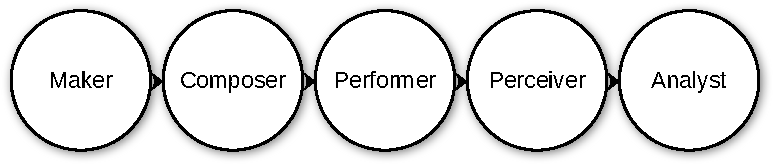
\includegraphics[width=\columnwidth]{figures/03-luthier-analyst-crop.pdf}
\caption{A linear, "feed-forward" process typically found in traditional musicking.}
\label{fig:music-quadrant1}
\end{figure}

The second role is that of the \emph{composer}, the person that creates the piece to be played. This role may or may not be closely related to the third role, the \emph{performer}, since composers may also play their own music. In some musical genres, particularly in those involving improvisation, the composition and performance processes may be wholly intertwined, what is sometimes called \emph{comprovisation} \citep{dudas_comprovisation_2010}. The same is true in many popular music styles, in which the music may be composed and performed by an artist or collectively by a band. From my simplified model's point of view, it still makes sense to include composition and performance as two separate processes. Separate study programs and professional organizations attest to composition and performance being seen as distinct roles in the music world.

The fourth role is often called `listener,' but I will refer to it as \emph{perceiver}. This is to stress that musicking is an embodied experience in which all modalities come into play. Listening---with the ears---is essential, but the sound of music is only part of a musical experience. As will be discussed more later, the other senses are also important, including seeing, smelling, and touching.

The fifth role is that of the \emph{analyst}, which includes the process of thinking and reflecting about musical experiences. This role should not be constrained to academic investigations of music. Any type of retrospective musical activity could fall into this category, including remembering a concert. Thinking about music---systematically or unsystematically---involves \emph{musical imagery}, what \citet{godoy_musical_2001} refer to as the ability to `hear' sound for your inner ear. This is something we all do, and which in itself may give rise to strong musical experiences.

Even though I have deliberately tried to separate the roles here, they certainly overlap. Some people may take on all the roles, albeit not at the same time. Others may take on two or three roles. As such, the roles are not mutually exclusive. Splitting them is an analytic approach to understand more about their inner workings. This will come in handy when we start investigating various types of instruments later.


\section{Music production}

To complicate things a little, I could add a sixth role: the \emph{music producer}. \citet[p. 5]{burgess_art_2013} defines music production as the `technological extension of composition and orchestration.' Thus on one side, we could consider the role of a producer as similar to that of a composer. That may be true for the role of many producers today. However, the first music producers were primarily doing live recordings of performances. Such recordings were made on the fly, and the recordists role could be considered close to that of a performer. They worked in real-time and only had one take. Today, we find a large variety of music producers, ranging from those running large-scale studios with many people involved to do-it-yourself singer--song-writers making complete albums in their bedroom \citep{jones_diy_2020}. There are also the producer-DJs going on stage, mostly working as performers \citep{kjus_live_2016}.

To generalize, I will, in the following, use music producer as an umbrella term to cover all aspects of what is often thought of as the \emph{art of record production} \citep{frith_art_2012}. This includes the engineering-oriented tasks of recording, mixing, and mastering. It also includes handling people and making artistic decisions at all stages throughout the process.
Today's music producers do not only passively record other's music; they are central in creating musical structures and shaping its \emph{sound} \citep{brovig-hanssen_digital_2016}. In Figure~\ref{fig:music-quadrant2}, I have, therefore, placed them somewhere between composers and performers.

\begin{figure}[tp]
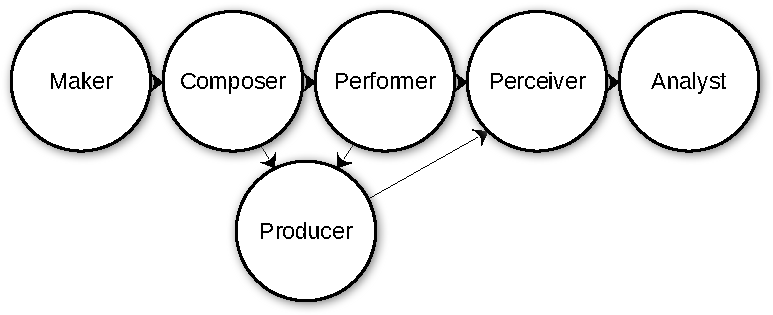
\includegraphics[width=\columnwidth]{figures/04-producer-crop.pdf}
\caption{The music producer can be placed between composers and performers in the chain.}
\label{fig:music-quadrant2}
\end{figure}

The role of music producers often overlaps with the other roles. Sometimes they have a distinct role alongside composers and performers. Other times, they may have double (or triple) roles as composers and performers. Still, it makes sense to separate the music producer's role from the composer and the performer. After all, they also have education programs, separate professional organizations, and follow different career paths.


\section{Creation versus experience}

One way of separating the different musicking roles is to see whether the activity in question is related to creative practice. I deliberately avoid talking about `active' and `passive' musicking here since one of the core elements of the musicking (and embodiment) paradigm is that everyone is actively engaged in one way or another. That is not to say that there are no differences between creating and experiencing music within a traditional musical context. I suggest thinking of them along a continuum, with creation on one side and experience on the other. Figure~\ref{fig:music-quadrant3} shows how it is possible to place the different actors in a grid with the experience--creation continuum on one side and time on the other. Here the temporal axis refers to when activities happen with respect to the `now' of a performance.

\begin{figure}[tp]
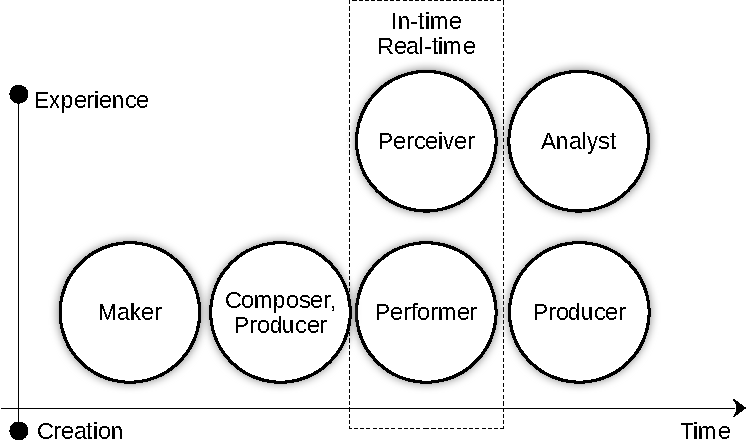
\includegraphics[width=\columnwidth]{figures/05-experience-creation-crop.pdf}
\caption{The different musicking roles may lean more towards either experience or creation. The temporal axis refers to the order of events with respect to the `now' of a performance.}
\label{fig:music-quadrant3}
\end{figure}

In this system, the instrument maker, composer, producer, and performer are placed on the creation side since they all create something (instrument, piece, performance, recording). A traditional perceiver and analyst will, in this system, be on the experience side. It is crucial, however, to think of one's placement along the continuum as dynamic. For example, a musician may perform during only one part of a concert while perceiving in others. Audience members may sit or stand still during parts of a performance but may also take on a more active role, such as singing or clapping. Understanding such dynamic role changes is essential to explain the complexities of real-world musicking.


\section{Temporal awareness}

Another way of looking at the different musicking roles is concerning time. Much has been written about how we experience music in time, see, for example, the works by \citet{kramer_time_1988,barry_musical_1990,london_hearing_2004,savage_music_2017,kozak_enacting_2019}, to mention a few. My approach to musical time is shaped by a techno-cognitive perspective, combining phenomenological and technological models of time.

\citet{dainton_temporal_2018} proposes to group different models of temporal awareness into three categories:

\begin{description}
  \item[Cinematic model:] our awareness is similar to that of taking `snapshots' of the continuous unfolding of time. An example is how the rapid projection of still images is perceived as a `moving image.'
  \item[Retentional model:] our awareness contains episodes of consciousness. These episodes contain a combination of the direct experience and representations (\emph{retentions}) of the past.
  \item[Extensional model:] episodes of an experience have a temporal extension and can be seen as extended \emph{chunks} of time.
\end{description}

As sketched in Figure~\ref{fig:cognition7}, the cinematic model can be seen as similar to how computers handle time. Digital computers sample the continuous data flow at regular time intervals. Each sample represents a moment in time without reference to its surroundings. Temporal fluidity in the playback of such independent samples is ensured through a high enough sampling rate. This way, our senses are `tricked' to believe that we watch or listen to a continuous phenomenon, even though the actual representation is a series of individual images or sound samples. Standard sampling rates---25~fps for video and 44.1~kHz for audio---are just about fast enough to `fool' our visual and auditory systems.

\begin{figure}[tp]
  \centerline{
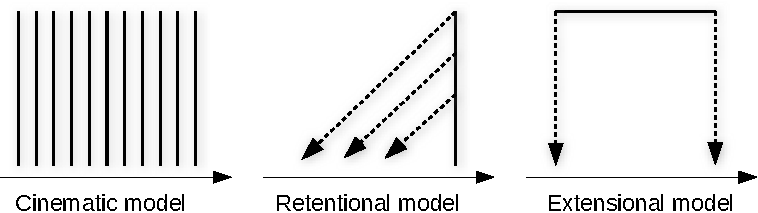
\includegraphics[width=\columnwidth]{figures/06-time-models-crop.pdf}
\caption{A sketch of the three main models of time consciousness: cinematic, retentional, and extensional, adapted from \citep{dainton_temporal_2018}.}
\label{fig:cognition7}
}
\end{figure}

The retentional and extensional models can be seen as ways of preserving a memory of the past. In the retentional model, one may think of what \citet{husserl_phenomenology_1991} called \emph{primal impressions} of a `now-point' in time. These primal impressions are always connected to what happened (\emph{retentions}). They also anticipate what will happen in the future (\emph{protentions}). In a discussion of the experience of the sound of an approaching coach, \citet[p. 290]{husserl_phenomenology_1991} writes:

\begin{quotation}
If we focus reflectively on what is presently given in the actually present now with respect to the sound of the postilion’s horn, or the rumbling of the coach, and if we reflect on it just as it is given, then we note the \emph{trail of memory} that \emph{extends} the now-point of the sound or of the rumbling. This reflection makes it evident that the \emph{immanent thing} could not be given in its unity at all if the perceptual consciousness did not also encompass, along with the point of actually present sensation, the continuity of fading phases that pertain to the sensations belonging to earlier nows.
\end{quotation}

In Husserl's model, the retentions are not the same as other types of memory; they are merely the gradually `fading away' of past `nows.' Using a signal processing metaphor, this may be thought of as a decaying delay line. What was once at the forefront of the signal gradually disappears.

Much has been written about the philosophy of time consciousness, but I will here make a jump to a more recent psychological model proposed by \citet{stern_present_2004}. As a psychotherapist, his focus is on creating tools he can use in a clinical setting. His concept of the \emph{present moment} can be seen as a combination of the retentional and extensional models. The aim is not to explain the continuous unfolding of time but rather to create a tool for talking about `nowness' in a clinical setting. A core feature of the present moment is that it has an extension in time. This temporal extension is typically up to around 3--5 seconds, which is the approximate limitation of our short-term memory \citep{snyder_music_2000}. A present moment is short, yet at the same time, rich in content. For Stern, it is also essential that the present moment is a `whole'---what is often called a \emph{gestalt} in the psychology literature---rather than being decomposed into smaller units. A present moment has both a `now' and a `here.' This is something we will get back to in discussions about spatiotemporal distance in Chapter~\ref{chap:hybrid}.

Stern uses the present moment as a core element of his therapeutical practice, getting clients to talk about and analyze such moments from memory. He also reflects on how the present moment is active in musicking \citep[p. 29]{stern_present_2004}:

\begin{quotation}
[\ldots] a musical phrase contains an immediate past and future. The form of the musical phrase is revealed and captured by the listener as the crest of the immediate present instant passes from the still resonating horizon of the past [\ldots] toward the anticipated horizon of the future [\ldots] Much of the charm of listening to music lies in the surprises that the composer provides by inventing final paths that surprise us but do not overly violate the implications we sensed.
\end{quotation}

If we `zoom' closer into the experience of music, \citet{godoy_reflections_2008} has suggested that we may not necessarily need to choose between the different awareness models; they may co-exist. He proposes to think of the perception of an unfolding temporal stimulus as a combination of continuously and discontinuously updated \emph{chunks}, as sketched in Figure~\ref{fig:cognition8}. This may work because it is not the beginning and end of the chunks that are of importance, but their \emph{goal points}. In music, such goal points can be individual tones or combinations of tones that form a chunk, for example, a musical phrase.

\begin{figure}[tp]
  \centerline{
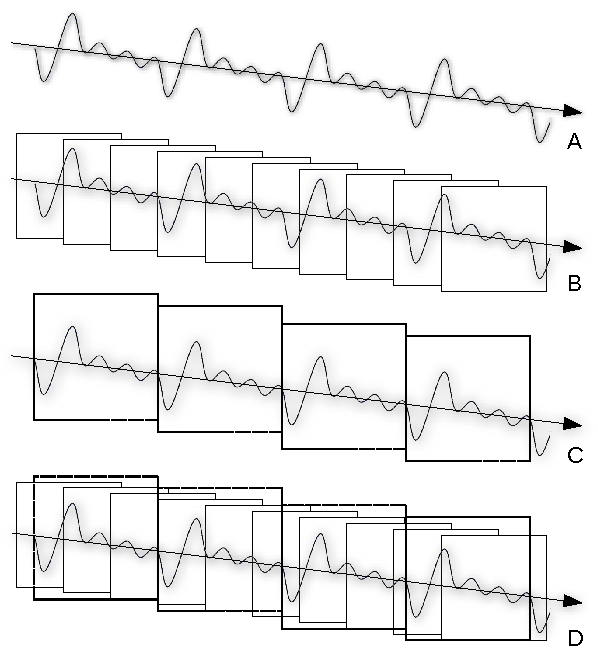
\includegraphics[width=0.7\columnwidth]{figures/07-time-windows-crop.pdf}
\caption{Three different types of awareness (B--D) based on a continuous sound signal (A): a floating time window (B), a discontinuous chunk-based updating (C), or a combination of B and C (D), based on \citep{godoy_reflections_2008}}
\label{fig:cognition8}
}
\end{figure}

From a techno-cognitive perspective, it is interesting to reflect on how a computer's time handling compares to the models of time awareness. As discussed above, sampling can be seen as similar to the snapshots of the cinematic model. However, recent digital representations are based on techniques similar to those of the retentional and extensional models. For example, video compression methods are based on storing \emph{keyframes} at regular intervals. These keyframes contain a complete image, while the following frames only contain information about the pixels that have changed from the keyframe. This is based on the technique of \emph{frame differencing}, meaning that subsequent frames are subtracted from each other. The resultant image only contains information about the changes between frames and can be used for motion analysis \citep{jensenius_methods_2018}. Such a keyframe-based compression technique results in much smaller file sizes than if all the images had to be stored entirely. We find similar methods used in compressed audio formats, such as MP3 and AAC, which use psychoacoustical models in the different temporal filters to reduce the size of audio files \citep{brandenburg_mp3_1999}. These multimedia formats are good examples of how knowledge about human psychology and cognition can help create better and more efficient technologies.


\section{The speed of time}\label{sec:time}

One aspect that we have not touched upon so far is the `speed' of time. This may be an odd topic from a cognitive point of view, but it is relevant when dealing with computers in which the processing speed is often a significant limitation. Broadly speaking, we can think about two temporal levels in computing systems: \emph{real-time} and \emph{non-real-time}. A real-time system is based on continuously taking in some input, performing the programmed calculations as quickly as possible, and then sending out the result. This is the way most electro-acoustic instruments work. From a cognitive perspective, it may be more relevant to talk about what \citet{wollner_slow_2018} refer to as `clocktime.' However, when balancing between cognitive and technological concepts, I have found it more useful to use the term real-time, since it will primarily be used when discussing technological issues.

Since a chain of operations necessarily takes some time, there is always some delay in a real-time computer-based system. The delay between a system's input to its output can be measured as the system's \emph{latency}. Sometimes the latency is below a perceptual or cognitive threshold, in which the technological imperfection does not matter from a perceptual point of view. Other times, the latency is evident to the perceiver but still tolerated. After all, we are used to compensating for various types of latencies, and, as argued by \citet{sethares_rhythm_2007}, several of them are also the basis for various perceptual phenomena and musical features (Figure~\ref{fig:time-sethares}). There are also cases in which latency is a significant problem, which we will discuss in Chapter~\ref{sec:latency}.

\begin{figure}[tp]
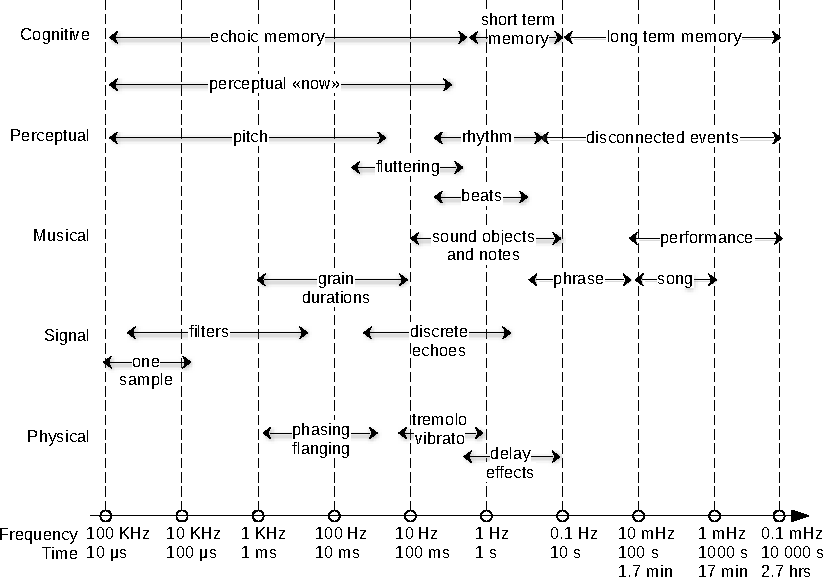
\includegraphics[width=\columnwidth]{figures/08-time-durations-crop.pdf}
\caption{A schematic overview of different temporal scales, adapted from \citep[p.7]{sethares_rhythm_2007}.}
\label{fig:time-sethares}
\end{figure}

The perception of latency is an example of the human ability to experience that something is not in time with the current `now.' For example, think of a thunderstorm. The lightning can be seen seconds before hearing the thunder. Still, you know that the thunder and lightning come from the same action, even though the vision and sound are experienced at different times. If you only hear the thunder, you will immediately think that you did not see the lightning. Moreover, when you see the lightning, you will wait to hear the thunder. But when does the lightning/thunder \emph{actually} happen? At the time you saw the lightning? When you heard the thunder? How do they relate to your sense of it happening in the `now'?

Let us move to a more musically relevant thought experiment. Imagine seeing someone pressing a key on a digital synthesizer without hearing any sound. One second later, you hear a sound. If no other sound-producing actions are made, you may perceive that the action and sound are related yet with a perceivable latency. What if the latency was one minute? Or one hour? Unless you were at an experimental concert during which the performer would wait for the sound with the audience, such sonic delays would be far beyond your latency tolerance. \citet{wessel_problems_2002} suggested ten milliseconds as the optimal target latency when developing electro-acoustic instruments. However, few computer-based instruments can meet such a `10-millisecond' requirement in practice. Yet, many instruments are still perceived as having tolerable latency levels. As illustrated in Figure~\ref{fig:time-sethares}, whether something is experienced as immediate or not in a musical context highly depends on the musical content.

Even though our latency tolerance may vary depending on content and context, it is quite clear that we have a sense of something being \emph{in-time} with the experienced `now.' Some events can also be considered \emph{out-of-time}, as sketched in Figure~\ref{fig:in-time}. This can be an action that happened in the past. Alternatively, it can also be a prediction or planning of something that will happen in the future. Scheduling is essential when creating computer-based systems, as they allow for preparing various actions that can be triggered based on the incoming signal.

\begin{figure}[tp]
  \centerline{
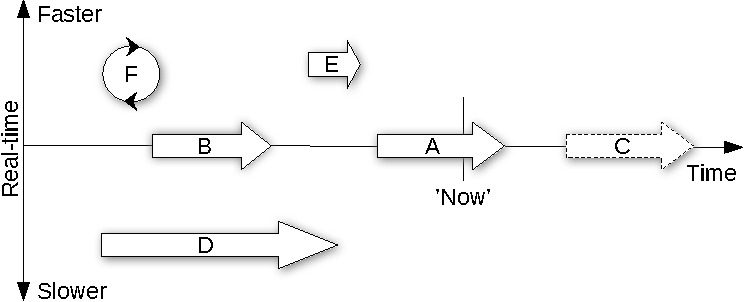
\includegraphics[width=.95\columnwidth]{figures/09-real-time-crop.pdf}
\caption{Relationships between different temporal levels. An event can happen in the `now,' both in-time and in real-time (A). We may also think of an event that happened in the past (B) or predict a future event (C). It is also possible to create slower (D) and faster (E) events with machines. Both conceptual and technological musical events may also be based on non-linear time, for example, circular time (F).}
}
\label{fig:in-time}
\end{figure}

When computers process in-time, we typically want them to also work in real-time. For example, if you set up a microphone with a reverb effect for a performance, you would like it to work in both in-time and real-time. However, if you just want to add reverb to a pre-recorded song, it does not matter when or how fast it happens. You may probably prefer that the computer does the processing \emph{faster-than-real-time}. If the computer can process a 3-minute sound file in 7 seconds, it is unnecessary to wait 3 minutes to finish its processing. You may also happen to have a computationally heavy reverb model that runs \emph{slower-than-real-time}. For a producer working in a studio, it is not crucial whether a process runs in real-time. For a performer on stage, however, there is no other option than running in real-time mode. The concert is happening in the `now,' hence the tools used need to run both in-time and real-time. Since there are so many different use cases and requirements, and time is so critical in music, it is not strange that computer music people talk a lot about latency issues. This is also one reason why there are many approaches to handling time in music programming languages \citep{dannenberg_languages_2018}.

\citet[p.3]{kozak_enacting_2019} argues that musical time can also be thought of independently from `objective' time:

\begin{quotation}
Imagine time differently, then---as a sphere, or a cube, or even a hexacosichoron. Imagine it running diagonally, or folding back upon itself, or sideways, or from the inside out. Imagine time crackling, wheezing, rustling, swooshing, buzzing. Imagine time as silent. Now imagine it smelling of freshly cut grass, or a musty hotel lobby. Then again, what if time glistened and shimmered? What if it breathed, slowly, in-out-in-out-in-out? What if it came near you, so close that you could feel its warmth, embrace it, hold it in your hands? What if it did all of that at once?
\end{quotation}

The idea is that musical time does not exist independently but is based on the interaction between musical sounds and moving bodies engaged in musical activities. This is an exciting line of thought and one that I would like to follow more in the future. However, in the context of this book, I will think of time in a more traditional sense. Still, given the techno-cognitive perspective, I will consider time as both objective and subjective at the same time.

A discussion about time---whether something is happening in-time or out-of-time, in real-time or non-real-time---only makes sense when we have a reference point: the `now.' The `now' is a subjective and relative entity. One might imagine that agreeing on a `now' should be easy for basic musical structures. However, recent rhythm studies have shown that even identifying the `beat' in individual tones is a non-trivial task \citep{danielsen_where_2019}. The task is much more difficult when one deals with complex music. I remember a concert in which a guitarist used a \emph{looper} in one of the songs, a device that can record and play short snippets of sound. When the performer came on stage, it was not immediately clear that she was using a looper since it was just one of many boxes in her setup. I was, therefore, puzzled when I could see her playing on the guitar without any sound coming out of the speakers. The guitar sound was routed into the looper, which recorded the first layer of the tune she was about to play. When she stepped on the looper's pedal to stop recording, the sound started playing. Here a temporal disruption of action and sound lead to a sense of an out-of-time performance. This was based on my reference point being the `now' of her performance action. A looper plays with the repetition of the `nows' of the past. Later in the same concert, the guitarist also started playing with the speed of the different sounds she recorded into the looper, making them faster and slower. This could be seen as the in-time use of real-time and non-real-time processing of the sound.

The case of the looping guitar is focused on relatively short time scales, but we may extend the ideas of in-time and real-time. Let us look at the roles of the musicking quadrant concerning a traditional concert with acoustic instruments. Then it is natural to consider that both the performer and perceiver are involved in in-time and real-time musicking.
If we use the `now' of the concert as the reference, then the performer's rehearsal of the concert program earlier the same day would be considered out-of-time. Similarly, one audience member's imagery of the performance (in the form of a mental `replay') later that day would also be considered out-of-time.
Similarly, we can argue that the instrument maker's role in making the instrument used in the performance is out-of-time concerning our imagined performance.

A composer's work would generally be considered out-of-time. The composition process would usually be slower than that of the final musical performance (slower-than-real-time). However, sketching out the form of an extended composition may happen quickly (faster-than-real-time). The composition process may also occur in real-time if the composer improvises a piece that is later written down and re-performed in concert. One such example is \emph{The Köln Concert} by Keith Jarrett, first performed in 1975 as extended piano improvisations. After popular demand, the concert was later notated and released as authorized sheet music \citep{jarrett_koln_1991}. What was at first an improvised performance is now played as a `composed' piece of music.

The temporal dimensions of the analyst's role are equally complex. It is common to start an analysis process as a perceiver. Still, music analysis is often carried out both out-of-time and slower-than-real-time concerning the performance one is studying. This could involve detailed listening and re-listening of certain parts of a piece of music to understand its harmonic or textural changes.

The complexity of all possible temporal combinations can be high. My interest is not to complicate things too much but rather to explain the general differences between in-time and out-of-time processes. This is also useful when expanding the model to include music production. For example, a live recording may be considered a separate (in-time) layer between the performer and the perceiver. However, as sketched in Figure~\ref{fig:music-quadrant2}, modern-day music production is often a much more circular process between the composer, performer, and producer. In such cases, the temporal complexities of a multi-layered model are high, with different layers of in-time and out-of-time processes overlapping. Such complexities are particularly noticeable when it comes to `live' music. As noted by \citet{danielsen_mediated_2016}, many pop music concerts are based on the playback of pre-recorded elements. As such, the liveness of the performance is built around the idea of creating a `mediated immediacy.' Audiences can accept significant discrepancies between what they see and hear if some of the music's core auditory elements are represented visually.


\section{Putting it all together}

\begin{figure}[tp]
  \centerline{
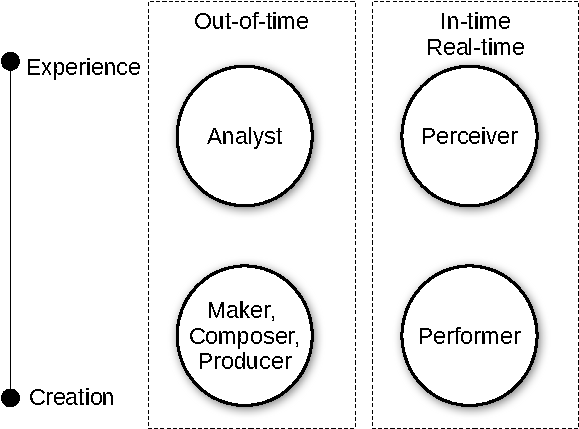
\includegraphics[width=.75\columnwidth]{figures/10-experience-creation2-crop.pdf}
\caption{The musicking quadrant, identifying four distinct types of musical engagement that can be placed along two axes: creation versus experience, and in-time and out-of-time processes.}
\label{fig:music-quadrant4}}
\end{figure}

After explaining its different components, we arrive at the complete model of the musicking quadrant, as sketched in Figure~\ref{fig:music-quadrant4}.
This model is, obviously, a coarse simplification and generalization of the complex reality of musicking. Nevertheless, it attempts to separate some quite distinct processes, roles, and products of today's music world. The musicking quadrant can also be used to understand more about how the traditional roles are changing. Today, machines enter all parts of the musicking quadrant. This is exciting, but it may also lead to some challenges, which we will discuss in later chapters.

The different roles in the musicking quadrant should not be seen as mutually exclusive. We have noticed an increasing level of specialization and professionalization in the music world over the last centuries. At the same time, there are also many examples of one person taking on several roles. One person could go and make a flute, come up with some idea for a song, and play it. This would then include the roles of instrument maker, composer, and performer. Another example of such a blending of roles is that of an `open-mic' session. Many of the people present here would partake in the musicking, both in the roles of performer and perceiver.

When it comes to the analyst role, I believe this should extend beyond the work by musicologists. Any type of musical reflection or thinking back at a performance would fall into this category in my model. Both the analyst and the perceiver are on the experiencing side of the musicking spectrum. The main difference is that the perceiver's experience is happening in-time (and real-time) with respect to the performance, while the analyst's activity is happening out-of-time (in either real-time or non-real-time). These may blend, however. An analyst may have been a perceiver at a concert and later re-listen to the performance from a recording. The latter would be an example of real-time listening, but out-of-time concerning the performance. The analyst can then do a non-real-time (and out-of-time) performance analysis using different music analytical tools.

As these examples show, it is easy to find combinations of the different roles of musicking in the world of traditional (acoustic) music. New roles appear with new technologies. The music producer is one such example. At first, this role was only concerned with physically recording music onto a fixed medium, in-time and real-time. Using new technologies, today's music producers largely overlap with composers and performers. In some cases, music producers also use advanced music analysis tools as part of their production chains. One such example is the use of pitch tracking software to align recorded sound with scores.

The advent of mobile phone apps for `active listening' makes it possible for perceivers to take on a performer role. The developer of those apps---the `digital luthier' to borrow a term from \citet{jorda_digital_2005}---is not any longer only an instrument builder, but could be seen as adding musical content like a composer. We will look more at such cases later and use the musicking quadrant to understand and define the roles. For those discussions, however, it may be more relevant to focus on \emph{processes} than actors: the functions of creating, performing, perceiving, and understanding music (Figure~\ref{fig:music-quadrant5}). In later chapters, we will look more closely at how these processes interact.


\begin{figure}[tp]
  \centerline{
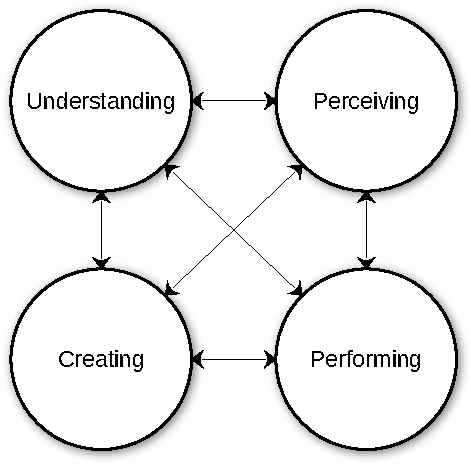
\includegraphics[width=.6\columnwidth]{figures/11-understanding-performing-crop.pdf}
\caption{Instead of talking about actors, we may think of the musicking quadrant as identifying four distinct types of musical engagement: creating, performing, perceiving, and understanding music.}
\label{fig:music-quadrant5}
}
\end{figure}
